% 电子管收音机
% 电子管收音机.tex

\documentclass[12pt,UTF8]{ctexbook}

% 设置纸张信息。
\input{../../../common/page}

% 设置字体，并解决显示难检字问题。
\xeCJKsetup{AutoFallBack=true}
\setCJKfamilyfont{hei}{SimHei}
\setCJKfamilyfont{kai}{KaiTi}

% 目录 chapter 级别加点（.）。
\usepackage{titletoc}
\titlecontents{chapter}[0pt]{\vspace{3mm}\bf\addvspace{2pt}\filright}{\contentspush{\thecontentslabel\hspace{0.8em}}}{}{\titlerule*[8pt]{.}\contentspage}

% 支持目录点击跳转
\usepackage[colorlinks,linkcolor=blue,citecolor=blue,urlcolor=blue]{hyperref}

% 设置 part 和 chapter 标题格式。
\ctexset{
	part/name= {第,卷},
	part/number={\chinese{part}},
	chapter/name={第,章},
	chapter/number={\arabic{chapter}}
}

% 图片相关设置。
\usepackage{graphicx}
\usepackage{float}
\graphicspath{{Images/}}

% 设置署名格式。
\newenvironment{shuming}{\hfill\zihao{4}}

% 注脚每页重新编号，避免编号过大。
\usepackage[perpage]{footmisc}

% 设置古文原文格式。
\newenvironment{yuanwen}{\bfseries\zihao{4}}

% 设置段落间距
\setlength{\parskip}{0.8em plus 0.2em minus 0.1em}

% 列表格式支持，列表项向右偏移。
\usepackage{enumitem}

% 数学公式支持
\usepackage{amsmath}

\title{\heiti\zihao{0} 电子管收音机}
\author{WangFei}
\date{\today}

\begin{document}

\maketitle
\tableofcontents

\frontmatter
\chapter{前言}

矿石收音机虽有其独特魅力，但其核心的矿石检波器灵敏度低且稳定性差，需要用细针在矿石表面仔细寻找灵敏点。如今我们制作矿石收音机时，通常用晶体二极管替代矿石检波器，但晶体二极管是半导体技术成熟后的产物，比矿石检波器晚出现数十年。在电子管诞生初期，人们只能依赖这种需要精心调试的矿石检波器。为了寻求更可靠的无线电信号检测方法，研究人员从电灯泡中获得了灵感。

\mainmatter

\part{真空二极管的诞生}

\chapter{从静电场到热电子发射}

\section{静电场的基本原理}

我们知道，在两个金属板之间加上直流电压，板间就会建立起静电场。如下图所示：

\begin{figure}[htbp]
    \centering
    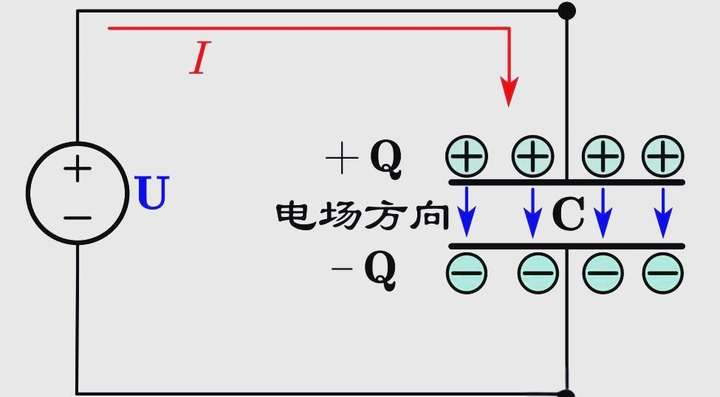
\includegraphics[width=0.7\linewidth]{electrostatic_field.jpg}
    \caption{平行金属板间的静电场}
    \label{fig:electrostatic_field}
\end{figure}

\section{热电子发射现象}

与此同时，物理学家还发现，当金属被加热到炽热状态时，它的表面会向外释放电子，这就是\textbf{热电子发射}，也叫\textbf{爱迪生效应}。

于是人们想到：如果将这两种现象结合会怎样？将平行金属板的负极替换为通电加热的灯丝，使其发射电子；正极板则保持静止等待接收电子。

整个装置要怎样保护？为了避免灯丝在空气中瞬间烧毁，也为了让飞出的电子不会撞上空气分子而散乱，人们把灯丝和金属板一起封进一个抽成高度真空的玻璃泡里。于是，\textbf{真空二极管}诞生了。

\section{电子管的真空度}

电子管内必须保持高度真空，不允许存在大量残余气体。如果残余气体过多，电子会与气体分子碰撞而降低运动速度，同时产生二次电子发射和气体电离，形成复杂的气体放电现象，干扰正常电子流。此外，残余气体会导致发射电子的电极氧化损坏。因此，电子管也被称为真空管。

电子管玻璃泡壁上常可见一层银色或黑色薄膜，这是抽空后利用吸气剂吸收残余气体留下的痕迹。吸气剂附着在电极后方的小金属杯或支架上，受热时与残余气体化合，形成这层薄膜。

\chapter{电子管的阴极结构}

根据释放电子的结构不同，电子管的阴极主要分为两种。

\section{直热式阴极}

第一种是\textbf{直热式阴极}：灯丝本身就是发射电子的阴极。通电后灯丝被加热至高温，电子直接从灯丝表面发射出来。这种结构简单直接，但由于灯丝同时承载加热电流，微小的电压波动会叠加在电子流上，容易引入交流哼声。

\section{旁热式阴极}

第二种是\textbf{旁热式阴极}。它将加热和发射功能分离：灯丝仅负责发热，外部套有涂覆特殊氧化物的金属圆筒，由圆筒发射电子。由于阴极与加热灯丝在电气上绝缘，阴极本身是等电位面，发射的电子流非常稳定，即使采用交流电加热也几乎没有干扰。后来绝大部分收音机和放大器使用的电子管都采用这种旁热式阴极。

\section{灯丝材料}

电子管的热电子发射来源于"灯丝"（又称丝极）。电流通过灯丝产生热量并发射电子。电子管常用的灯丝材料包括：

（1）\textbf{钨丝灯丝} 和普通电灯泡的灯丝一样用钨丝做成，坚固耐用，在2400°C时发射性能最好，但需要消耗较大的功率，所以不太经济。

（2）\textbf{钍层灯丝} 在钨里面加入一些氧化钍，经过特别处理之后，钨丝表面就覆盖一层薄钍膜，可以在较低的温度下发射大量电子。当1000°C时发射的电子，就和同面积的钨丝在2000°C时所发射的电子数量相等。不过在灯丝过热或电压过高时，钍层会损坏失效，不再发射电子。

（3）\textbf{碳化层灯丝} 是钍层灯丝经过萘蒸气或乙炔蒸气的热处理，在表面产生一层碳化钨，能够将钍层原子固定起来，不易蒸发，工作温度也只有1800°C。不过性质较脆，在经常移动的收音机中使用时，灯丝容易因振动而折断。

（4）\textbf{涂钍灯丝} 它是在钨丝外涂一层氧化铜，再涂一层钍而成。所需工作温度不高，发射效率也高，不会因过热而失效，是一种比较可靠的灯丝。

（5）\textbf{氧化层灯丝} 它是在铁镍合金（或其他化合物）制成的灯丝上，涂一层钡或锶的碳酸盐，在较低温度下（约650-850°C）就能发射大量电子，所以又叫做"活化灯丝"。性能比钍层灯丝更稳定，现在小型收音机中所用的电子管，绝大部分采用这种经济高效的活化灯丝。

\chapter{真空二极管的工作原理}

\section{二极管的基本结构}

二极管是最简单的电子管。它是在灯丝外面围绕一块金属板，封装在真空玻璃泡内。灯丝是一个电极，金属板是另一个电极。因为金属板的形状像一个屏风，所以叫它做"屏极"（或板极）；又因它通常加正电压，故又叫阳极。这种只有两个电极的电子管，叫"二极管"。各电极通过导线引出管外。

\begin{figure}[htbp]
    \centering
    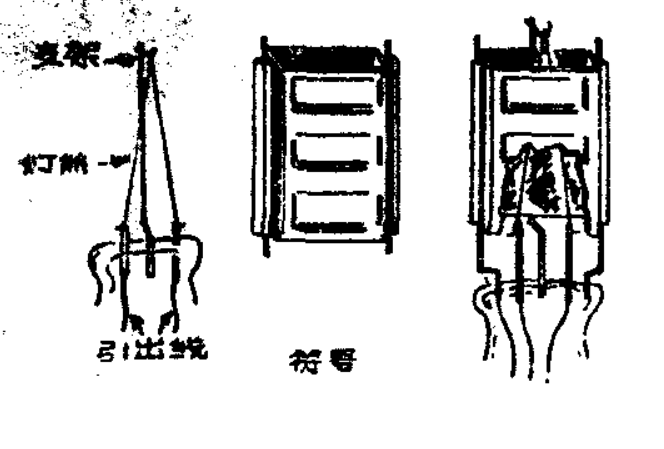
\includegraphics[width=0.7\linewidth]{diode_structure.png}
    \caption{二极管的构造}
    \label{fig:diode_structure}
\end{figure}

\begin{figure}[htbp]
    \centering
    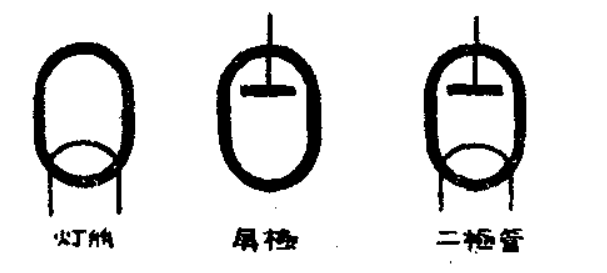
\includegraphics[width=0.5\linewidth]{diode_symbol.png}
    \caption{二极管符号}
    \label{fig:diode_symbol}
\end{figure}

\section{二极管的单向导电性}

二极管工作时需要两组电源：一组为灯丝（直热式阴极）供电，称为"甲电"，电流通过灯丝产生热量使其发射电子；另一组为屏极提供工作电压，称为"乙电"，其正极接屏极，负极接阴极。

当乙电正确连接时，屏极带正电，与阴极之间形成电场。从阴极飞出的电子被带正电的屏极吸引，形成从阴极流向屏极的电子流——称为"屏极电流"或"屏流"。电子到达屏极后，经乙电回路返回阴极，形成完整的"屏极电路"。

如果将乙电反接，屏极将带负电。此时，带负电的屏极会排斥同样带负电的电子，电子无法到达屏极，屏流无法形成。若移除乙电，屏极不带电，虽有少量高初速度电子可能到达屏极形成微弱电流，但只有当屏极带负电时才能实现完全截止。

这种\textbf{单向导电性}（电流只能从阴极流向阳极）是真空二极管的核心特性，使其成为理想的单向导电阀。这一特性有两大重要应用：一是在无线电接收中用于检波——当调谐电路将已调好的高频电流送到屏极时，正半周时屏极带正电，检波电路有电流通过；负半周时屏极带负电，电子流被排斥，电流不通。经过听筒的电流成为脉动直流，其振幅与输入的高频电流相同，因此能听到播音。二是用于整流——将交流电转换为直流电，这在电源供应设备中至关重要。

\begin{figure}[H]
    \centering
    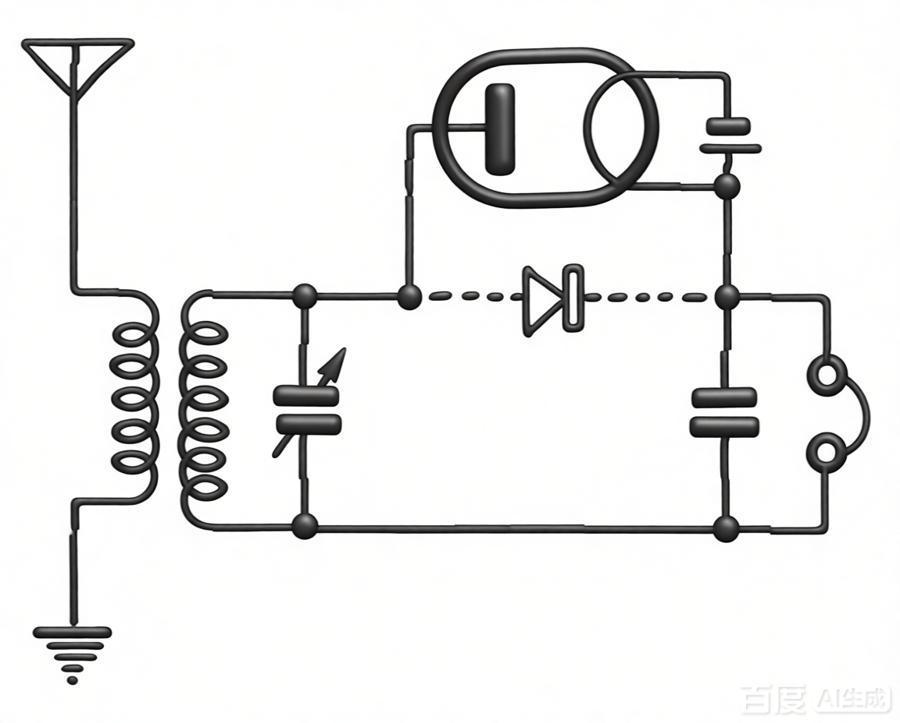
\includegraphics[width=0.8\linewidth]{diode_detector_circuit.jpg}
    \caption{二极管检波电路}
    \label{fig:diode_detector_circuit}
\end{figure}

二极管检波器的最大优势是工作稳定，不像矿石检波器那样因灵敏点接触变化而影响收音效果。但其缺点也很明显：灯丝需要消耗电能，且本身没有信号放大能力，通过听筒的仍是天线上的微弱电流，音量无法提升。

弗莱明发明的这一器件被称为"弗莱明阀"，标志着电子管时代的开端。但要实现真正实用的无线电接收，还需要能够放大微弱信号的器件——这正是真空三极管要解决的问题。

\section{各极电压与屏极电流的关系}

各极电压与屏极电流的关系如下：

当屏极电压保持不变时，改变灯丝电压会影响屏极电流：电压升高使灯丝温度上升，电子发射量增加，屏极电流随之增大；反之，降低甲电电压会使灯丝温度降低，电子发射量减少，屏极电流随之减小。但这种做法会缩短灯丝寿命，甚至导致烧毁。因此，实际应用中灯丝电压都有额定值，灯丝的电子发射能力保持恒定。

在灯丝电压固定的情况下，改变屏极电压会对屏流产生影响：当乙电电压增加时，屏极吸收电子的能力增强，屏流随之增加。但由于灯丝发射的电子数量有限，当所有电子都被屏极吸收后，再增加屏压也不会使屏流继续增大，此时的屏流称为\textbf{饱和屏流}。

当降低屏极电压时，屏流随之减少。此时并非所有电子都被吸收，未被吸收的电子会聚集在阴极附近，形成带负电的"电子雾"。这些积累的电子被称为\textbf{空间电荷}，它们会产生排斥电场，限制阴极继续发射电子。即使阴极持续发射新电子，空间电荷区域也会迅速达到动态平衡，新发射的电子会补充被吸收的电子位置。

"电子雾"的分布与屏极电压和阴极电压都有关系。在屏极电压固定的情况下，若降低阴极电压，电子发射量减少，屏极能够吸收全部电子，此时不存在空间电荷；若提高阴极电压，电子发射量增加，空间电荷会显著增多。但由于空间电荷会排斥新发射的电子，其总量不会无限增大，而是达到动态平衡。

空间电荷会阻碍屏极吸收电子。为了克服这种阻碍，需要提高屏极电压以增强对电子的吸引力，这会导致功率消耗增加。因此，空间电荷对电子管的工作是有害的。

\part{真空三极管与电子学时代}

\chapter{真空三极管的发明}

这一关键突破来自美国发明家德·福雷斯特。1906年，他在二极管的阴极和阳极之间引入了第三个电极——用金属丝制成的栅网状或螺管形结构，将阴极包围起来，称为\textbf{控制栅极}。这一新型器件被称为\textbf{真空三极管}。

\section{栅极的控制作用}

栅极的加入是一项革命性的创新。它位于阴极附近，处于电子从阴极飞向阳极的路径上。由于栅极与阴极距离很近，即使在栅极上施加很小的电压变化，也能显著改变阴极附近的电场分布，从而精确控制电子管内的电子流。这类似于通过微调水龙头阀门来控制水流大小——加在栅极上的微弱信号可以在阳极电路中产生波形相同但幅度显著放大的信号，\textbf{信号放大功能}由此实现。

三极管工作时除了甲电和乙电，还需要在栅极与阴极之间接入第三组电源——通称"丙电"，形成"栅极电路"。当丙电正极接栅极使栅极带正电时，它与带正电的屏极产生合成电场，增强屏极对电子的吸引力，使屏流增加；同时会有一小部分电子被栅极吸收，形成"栅极电流"。若将丙电反接使栅极带负电，其电场与屏极相反，削弱屏极吸引力，屏流减少，且栅极排斥电子不会产生栅极电流。当栅极负电压足够大时，排斥力超过屏极吸引力，电子无法到达屏极，屏流完全截止。

栅极正电压过高时，全部发射电子被栅极和屏极吸收，再增加栅压屏流也不再增加，此时达到"屏流饱和点"；栅极负电压过高时，全部电子被拒斥，屏流被切断，此时的丙电电压称为"切断负压"。

如果将交流电压输入栅极，当它的最大值在正半周不超过屏流饱和点、负半周不低于屏流切断点时，这种正负变化就能使屏极电流产生相应变动，如图\ref{fig:grid_voltage_waveform}所示。

\begin{figure}[htbp]
    \centering
    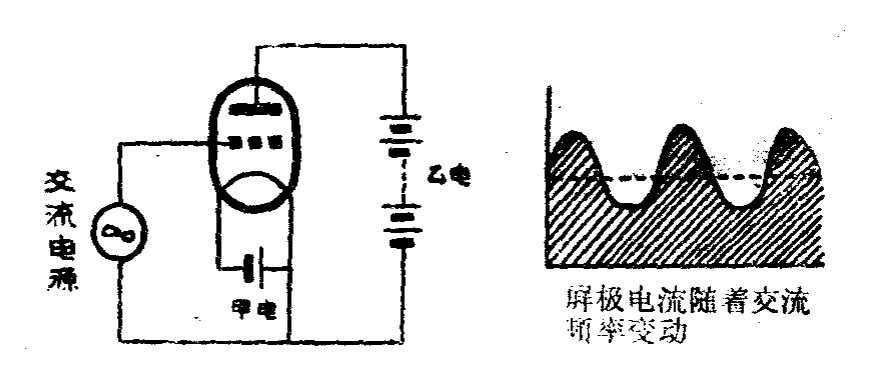
\includegraphics[width=0.7\linewidth]{grid_voltage_waveform.png}
    \caption{栅极电压与屏极电流波形}
    \label{fig:grid_voltage_waveform}
\end{figure}

栅极距离阴极的位置比屏极近得多，因此用相同电压分别加到栅极和屏极时，栅极产生的电场对电子的控制能力远强于屏极电场。具体来说：栅极电压的微小变化就能引起屏流的显著变化，而若要通过改变屏极电压达到相同效果，则需要大得多的电压变化。因此，栅极的作用可以理解为：栅极上较小的电压变动，便能使屏流发生很大变化，所以栅极有时也被称为"控制栅"。

当栅极用于控制屏流时，通常会施加一个较小的负电压，这能使电子管工作在良好的特性区域，并且避免栅极吸收电子而消耗功率。这个电压称为"栅偏压"（或丙电压）。

\section{三极管的基本功能与影响}

由于三极管栅极的控制作用，这类电子管能够实现检波功能，对高频和低频信号进行放大，还能产生振荡。这些基本功能具有多样化且突出的特性，使得微弱的无线电信号可以被多级放大以驱动扬声器，稳定的高频振荡电路得以实现为无线电台载波发射奠定基础，长途电话信号放大成为可能，电视和雷达等新技术的研究也随之展开。

从收音机的普及和广播事业的兴起，到早期电子计算机的发展和现代电子工业的建立，真空三极管都起到了奠基性的作用。德·福雷斯特的这一发明开创了电子学的新时代。

\chapter{三极管的基本电路}

所有三极管电路都可以分为三个基本电路：阴极电路、栅极电路（又叫输入电路）和屏极电路（又叫输出电路）（图\ref{fig:triode_circuit}）。三个电路的公共点0叫做电路的"零点"。

\begin{figure}[htbp]
    \centering
    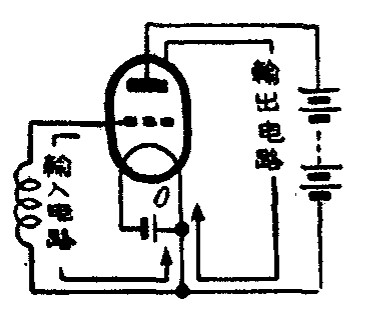
\includegraphics[width=0.7\linewidth]{triode_circuit.jpg}
    \caption{栅极电路和屏极电路}
    \label{fig:triode_circuit}
\end{figure}

因为屏极通常接正电压，所以有时叫它"阳极"；相对于阳极而言，发射电子的阴极也叫做"阴极"。

三极管是无线电技术里最基本的电子管，它的各种作用和实际应用，我们将在下面和以后逐一讲到。

\chapter{三极管的检波作用}

三极管的检波作用比二极管优良得多，这里介绍两种常用的三极管检波方法——屏极检波和栅极检波。

\section{屏极检波}

利用三极管的屏极电路进行检波工作的，叫做屏极检波法。电路如图\ref{fig:plate_detector}所示。在栅极接上一个丙电，使它带有相当高的负电压。在没有信号从调谐电路输入时，屏流将被截断。

\begin{figure}[htbp]
    \centering
    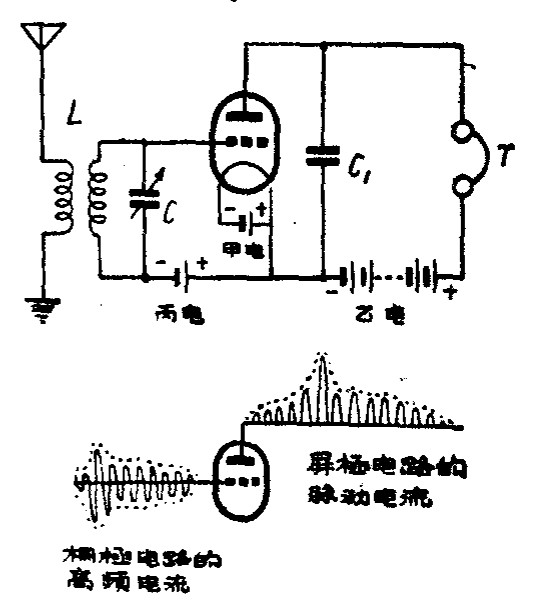
\includegraphics[width=0.7\linewidth]{plate_detector.jpg}
    \caption{屏极检波电路}
    \label{fig:plate_detector}
\end{figure}

调谐电路与栅偏压电源（丙电）串联。当输入信号处于正半周时，信号电压抵消了一部分栅极负偏压，产生屏极电流，其大小随输入信号幅度变化。当信号进入负半周时，信号电压与栅极负偏压叠加，使栅极负电压增大，从而切断屏极电流。将耳机串联在屏极电路中，正半周时有半周屏流通过，负半周时无电流通过。这样耳机中就产生了脉动电流，其幅度随输入信号变化，驱动耳机振膜振动发声。

屏极检波是在屏极电流上取得半周电流来完成检波工作的。这半周电流的变化与输入信号的音频变化相同，但幅度远大于输入信号，因此耳机发声较为响亮。

检波后残余的高频电流通过与耳机并联的"旁路电容器"（$C_1$）滤除，使耳机中只流过音频电流。

屏极检波虽然可以获得较大的输出电压，但灵敏度较低，仅在输入信号电压较大时使用。

\section{栅极检波}

利用三极管的栅极电路进行检波工作的方法，叫做栅极检波法。在栅极电路中，栅极不接入负电压，调谐电路与栅极之间连接一个"栅极电容器"（$C_1$）。输入信号的高频电流经过它到达栅极；在正半周时，栅极带正电吸收电子，但电子不能通过$C_1$完成回路，导致栅极上积存大量电子，阻碍屏极电流。因此需要在栅极和阴极之间接入一个电阻（$R$），使一部分电子通过它漏泄回阴极，这个电阻称为"栅漏电阻"。

正半周时$R$上有电流通过，负半周时栅极带负电排斥电子，$R$上没有电流。于是栅漏电阻上产生的电压降就是一个与广播信号相似的脉动电压，残余高频成分仍可从$C_1$通过。

栅极电路相当于起着二极管检波的作用（此时的栅极相当于二极管检波时的阳极），结果在栅极上形成了高频电压和音频脉动电压的叠加。

\begin{figure}[htbp]
    \centering
    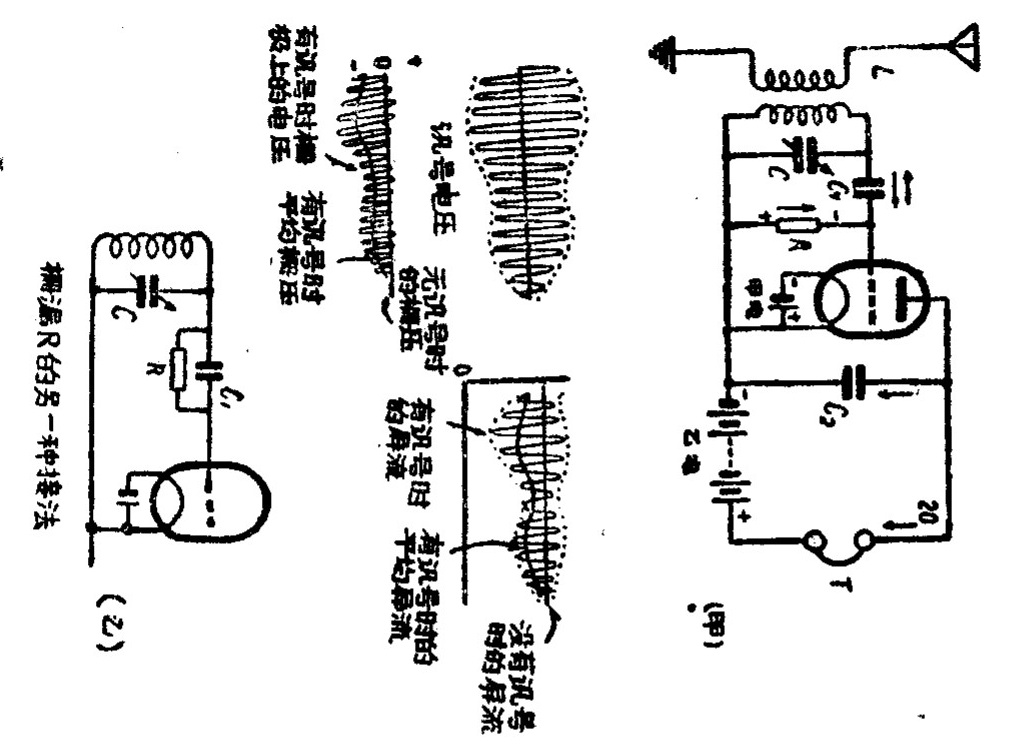
\includegraphics[width=0.8\linewidth]{grid_detector.jpg}
    \caption{栅极检波电路}
    \label{fig:grid_detector}
\end{figure}

屏极电路中，屏极电流受到栅极控制。当栅极起到二极管检波作用时，屏极电路中也会发生栅极上所有高频和音频成分的变化。高频电流从旁路电容器（$C_2$）流过后，耳机里流过的就是音频电流了。音频电流的变化与输入信号相同，但幅度要大得多。

栅极检波就是先在栅极电路检波，再在屏极电路放大。此法输出电压虽不很大，但相当灵敏，是简单电子管收音机中最常采用的电路。

栅漏电阻（$R$）有时也可与栅极电容器（$C_1$）并联，接法如图\ref{fig:grid_detector}所示，效果与图甲的接法相同。

\chapter{电子管收音机与多极管}

\section{电子管收音机的优势}

采用电子管作为检波器后，收音机的灵敏度和选择性显著提升，性能远超矿石收音机。

尽管电子管收音机需要电源供电，但单管收音机的功耗较低，不会给普通用户带来显著的经济负担，因此这并非其主要缺点。

\section{多极管}

三极管是基本的电子管，用它几乎可以说明许多无线电电路的工作原理。虽然现在一般电路中大多采用效率更优的多极电子管，但它们都是在三极管的基础上改进而来，电路原理大同小异。

\subsection{四极管}

在屏极和栅极之间加入一个稀疏的网状电极，就构成了四极管。这个电极的作用是将屏极和栅极隔离开来，称为"帘栅"或"障栅"（图\ref{fig:tetrode_structure}）。在电路中，通常将它接入一个低于或相当于屏极的正电压，因此它也能吸收电子产生"帘栅电流"。不过由于它是稀疏的栅网，吸收电子的数量有限，大部分电子仍被屏极吸收。

帘栅在屏极前方产生一个强大的电场，对空间电荷有直接影响，从而减弱了屏极对空间电荷的作用，使得屏极电压的变化对屏极电流的影响减小。结果是控制栅对屏极电流的影响相对增大，即控制栅的效率得到了提高。

\begin{figure}[htbp]
    \centering
    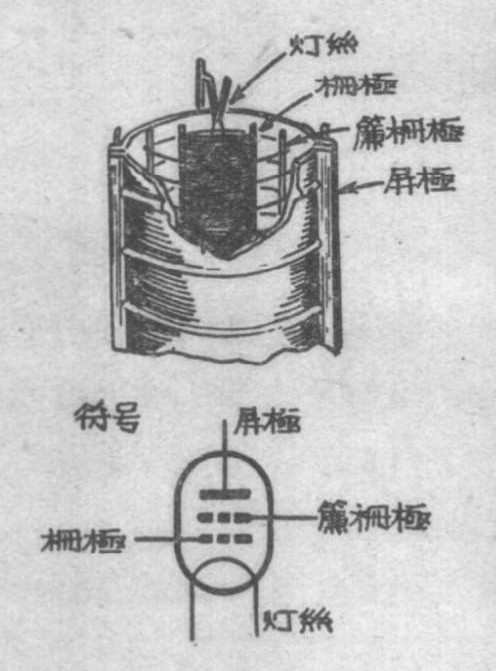
\includegraphics[width=0.7\linewidth]{tetrode_structure.jpg}
    \caption{四极管结构}
    \label{fig:tetrode_structure}
\end{figure}

其次，三极管中各个电极之间都可看作是微小的电容器，虽然电容量很小，但在高频工作时仍会产生影响，尤其是屏极和栅极之间的电容影响最大（图\ref{fig:interelectrode_capacitance}）。加入帘栅后，将屏极和栅极分隔开，形成两个串联的电容器，从而将总电容量降到很低，因此四极管在高频工作时性能远优于三极管。

\begin{figure}[htbp]
    \centering
    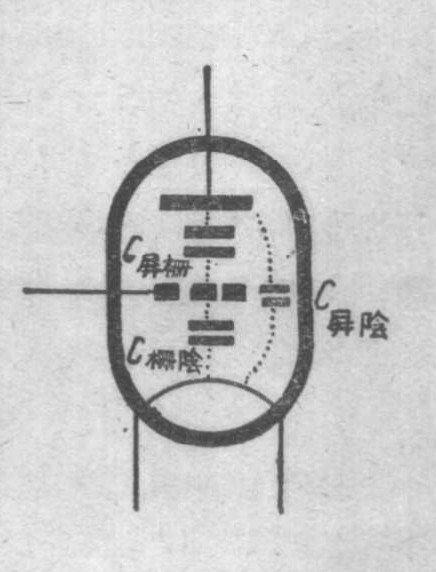
\includegraphics[width=0.7\linewidth]{interelectrode_capacitance.jpg}
    \caption{极间电容示意图}
    \label{fig:interelectrode_capacitance}
\end{figure}

然而四极管也有显著缺点：由于帘栅的存在使电子流加速，当高速电子冲击屏极时，会撞击出屏极的电子，形成二次电子发射。这些二次电子若能立即被屏极吸收回去影响不大，但电子管工作时，屏极电压有时会低于帘栅电压，此时二次电子会被帘栅吸收，导致帘栅电流迅速上升，同时到达屏极的电子减少，屏极电流下降，使电子管工作不稳定。

这个缺点使得四极管在收音机中应用较少。

\subsection{五极管}

为了克服四极管的缺点，设计者在屏极和帘栅之间再加入一个新的栅极，称为"抑制栅"或"遏止栅"（图\ref{fig:pentode_structure}）。它通常与阴极相连，电位为零，成为屏极和帘栅的静电隔离层。当发生二次电子发射时，抑制栅能将电子排斥回屏极，从而抑制帘栅吸收二次电子，大幅提高电子管的性能。

\begin{figure}[htbp]
    \centering
    %\includegraphics[width=0.7\linewidth]{pentode_structure.jpg}
    \caption{五极管结构}
    \label{fig:pentode_structure}
\end{figure}

五极管适用于各种放大工作，是目前最流行的电子管之一。

五极管的符号如图\ref{fig:pentode_symbol}所示，其结构特点是：最靠近阴极的栅极是控制栅（又称第一栅）；其次是帘栅（又称第二栅）；靠近屏极的是抑制栅（又称第三栅）。

\begin{figure}[htbp]
    \centering
    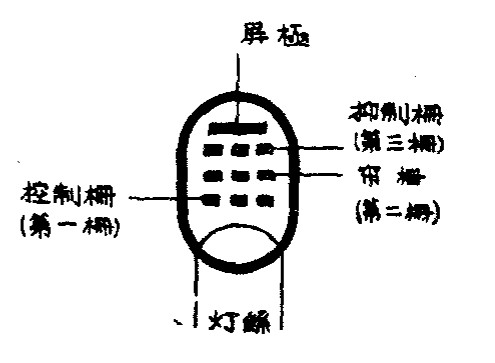
\includegraphics[width=0.5\linewidth]{pentode_symbol.jpg}
    \caption{五极管符号}
    \label{fig:pentode_symbol}
\end{figure}

\subsection{集射式四极管}

另一种能够克服二次电子发射影响的电子管是"集射式"四极管。普通阴极发射电子时是向四周扩散的；集射式电子管则在帘栅和屏极之间相对放置一对金属板，称为"电子束形成极"。它与阴极连接处于零电位，两边各留出一个"缺口"。电子从阴极发射出来后被这两块金属板排斥，只能集中从"缺口"冲出，形成一束强烈的电子流。

另一方面，栅极和帘栅的圈数相同且每圈彼此相对，电子束冲出时由于栅极带负电而被分成一排排，帘栅恰好处于每排电子束的"间隙"中，吸收电子的机会大为减少。同时，因电子集中在若干束内，在屏极前密度很大，能够将屏极射出的二次电子赶回屏极，避免被帘栅吸收。

集射式四极管的构造和工作情形如图\ref{fig:beam_tetrode}所示。电子束形成极在这里只作为辅助电极，因此这类电子管仍属于四极管。

\begin{figure}[htbp]
    \centering
    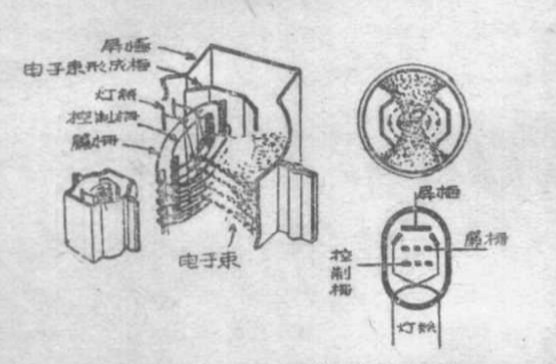
\includegraphics[width=0.8\linewidth]{beam_tetrode.jpg}
    \caption{集射式四极管的构造}
    \label{fig:beam_tetrode}
\end{figure}

在许多情况下，集射式四极管可以代替强力五极管，且性能更优。这类电子管在我国也有称为"束流管"、"集流管"或"电子注管"等名称。

\subsection{复合管}

有时为了使用方便和节省空间，可以将两个（或几个）电子管合装在一个真空玻璃泡内，称为"复合管"。大多数复合管还可以共用一个公共阴极，但管内每个"电极组"的作用仍然各自独立，不会相互影响。在后续的多管收音机中，我们也会使用到复合管。

\section{常用电子管的型式}

电子管的制造有多种不同的结构形式，在安装技术中需要充分了解它们的安装方法。下面列举一些常用的和国产的电子管型式。

\subsection{玻璃式}

这类电子管的外壳由玻璃制成，固定在一个胶木的"管腰"上。各电极通过导线从管内引出，焊接在管腰下方的"管脚"（插脚）内，以便插入"管座"（图\ref{fig:glass_tube}）。由于电极数目不同，插脚数目也不同，通常分为4脚式、5脚式、6脚式和7脚式四种。有时控制栅从管子顶部引出，连接在金属"管顶"上。这种型式在老式收音机中还能见到，但近来已很少使用。

\begin{figure}[htbp]
    \centering
    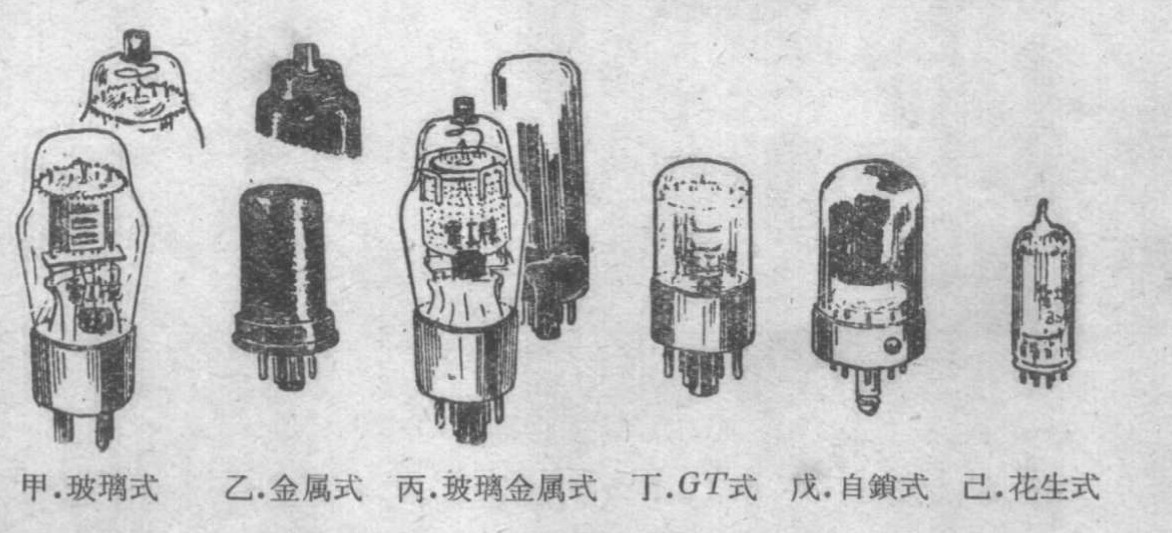
\includegraphics[width=0.7\linewidth]{glass_tube.jpg}
    \caption{玻璃式电子管（图甲）}
    \label{fig:glass_tube}
\end{figure}

\subsection{金属式}

金属式电子管在制造上更为先进。外壳用铁皮制成，因此无法窥见内部结构（图\ref{fig:metal_tube}）。这种结构能隔离电子管与外界的不必要感应，散热更容易，体积也更小，内部接线可以缩短。不过内部电极的支持座和抽气口仍用玻璃制造，长期使用中由于冷热交替，玻璃与金属的结合处可能会产生漏气现象，导致电子管效率降低或失效。

\begin{figure}[htbp]
    \centering
    %\includegraphics[width=0.7\linewidth]{metal_tube.jpg}
    \caption{金属式电子管（图乙）}
    \label{fig:metal_tube}
\end{figure}

金属式电子管的另一个特点是：不论内部电极多少，插脚一律采用"八脚式"，其中有一个"对正键"，便于插入管座时不会插错。

但使用干电池作为甲电电源的电子管，几乎没有金属式的。

\subsection{玻璃金属式}

将金属式电子管的外壳改为玻璃材质，就成为玻璃金属式电子管（图\ref{fig:glass_metal_tube}），通常称为"G"式管。其内部电极构造和插脚排列与金属式完全相同，只需在金属管型号后加一个"G"字。例如：金属管6F6改为这种型式，就叫做6F6G。苏联的这类电子管则在型号后加一个"C"字，例如金属管6Ф6的玻璃金属式就是6Ф6C。

\begin{figure}[htbp]
    \centering
    %\includegraphics[width=0.7\linewidth]{glass_metal_tube.jpg}
    \caption{玻璃金属式电子管（图丙）}
    \label{fig:glass_metal_tube}
\end{figure}

\subsection{GT式}

玻璃金属式电子管体积与玻璃式一样较为笨重，后来制造商将其缩小到与金属式差不多的尺寸，称为"GT"式（图\ref{fig:gt_tube}），型号后加GT两个字母。例如：6F6G制成这种型式，就叫做6F6GT（苏联同类型管子后加-M字，例如6Ф6M、6Ф5M等）。

在我国有些地方，这种型式也被称为"小鸡式"。

\begin{figure}[htbp]
    \centering
    %\includegraphics[width=0.7\linewidth]{gt_tube.jpg}
    \caption{GT式电子管（图丁）}
    \label{fig:gt_tube}
\end{figure}

\subsection{自锁式}

自锁式电子管的玻璃泡与GT式相似，但管腰较矮，由金属制成，上面有一个圆点突出作为插入管座的标记。各电极的支柱直接伸出作为插脚，也是八脚式（但与上述八脚式不同）（图\ref{fig:self_locking_tube}）。对正键的末端有一圈小槽，插入管座后会被管座上特制的弹簧套住，不易跳出，因此称为自锁式（苏联这类电子管型号后带一个"Л"字）。

\begin{figure}[htbp]
    \centering
    %\includegraphics[width=0.7\linewidth]{self_locking_tube.jpg}
    \caption{自锁式电子管（图戊）}
    \label{fig:self_locking_tube}
\end{figure}

\subsection{花生式}

在常用电子管中，花生式的体积较小，整体由玻璃制成，尺寸约为一颗花生大小（图\ref{fig:peanut_tube}），插脚一律为7只。苏联同类电子管称为"姆指管"，型号后带一个"П"字。

\begin{figure}[htbp]
    \centering
    %\includegraphics[width=0.5\linewidth]{peanut_tube.jpg}
    \caption{花生式电子管（图己）}
    \label{fig:peanut_tube}
\end{figure}

\section{电子管的分类和电子管特性表}

电子管应用非常广泛，且有各种型式，种类繁多。通常按型式、构造、用途等进行分类（从前还有以其他方式分类的）。

每一种型号的电子管都有其独特特性，为了参考方便，通常按一定方法（如字母顺序、数字）排列，将它们的性能列成表格，称为"电子管特性表"。在特性表上，可以查找每一种电子管的各种数据、性能以及管座接线图等，非常方便。

不同国家的电子管命名体系有所不同。有些国家的电子管型号命名较为复杂，存在一定的重复。而苏联的电子管型号按照统一的全苏标准制定，每个字母和数字都表示特定意义，使用起来较为方便。

\subsection{苏联电子管命名规则}

苏联电子管型号通常由四部分组成：

\begin{enumerate}
    \item \textbf{第一部分（数字）}：表示灯丝电压（单位：伏特）
    \item \textbf{第二部分（字母）}：表示电子管型式（程式）
    \item \textbf{第三部分（数字）}：表示厂家特定的序号
    \item \textbf{第四部分（字母）}：表示构造型式
\end{enumerate}

其中第二个字母的含义如下：
\begin{description}
    \item[Д] 二极管
    \item[П] 输出五极管及集射管
    \item[Х] 双三极管
    \item[Г] 附二极管的三极管
    \item[С] 三极管
    \item[Б] 附二极管的五极管
    \item[К] 遥截止管
    \item[Н] 双三极管
    \item[Ж] 锐截止五极管
    \item[Ф] 三极-五极管
    \item[А] 双控制栅变频管
    \item[Л] 整流管
\end{description}

第四个字母表示构造型式：
\begin{description}
    \item[М] 金属玻璃式管（即GT式）
    \item[С] 玻璃管
    \item[Л] 自锁式
    \item[П] 姆指管（花生式）
    \item[Б] 超小型管（直径10公厘）
    \item[А] 特小型管（直径6公厘）
\end{description}

金属管则无第四个字母。

\subsection{中国电子管命名规则}

我国电子管命名体系参考了苏联标准并结合实际情况制定，型号通常由三到四部分组成：

\begin{enumerate}
    \item \textbf{第一部分（数字）}：表示灯丝电压（单位：伏特）
    \item \textbf{第二部分（字母）}：表示电子管类型
    \item \textbf{第三部分（数字）}：表示产品序号
    \item \textbf{第四部分（字母，可选）}：表示结构形式或改进型号
\end{enumerate}

常见的第二个字母含义：
\begin{description}
    \item[D] 二极管（如6D1、6D2）
    \item[C] 三极管（如6C1、6C2）
    \item[N] 双三极管（如6N1、6N2）
    \item[P] 五极管（如6P1、6P6P）
    \item[Z] 整流管（如6Z4、5Z3P）
    \item[F] 锐截止五极管（如6F1、6F2）
    \item[S] 束射四极管（如6S6）
\end{description}

常见型号示例：
\begin{description}
    \item[6P1] 6V灯丝，五极管，序号1
    \item[6N1] 6V灯丝，双三极管，序号1
    \item[6Z4] 6V灯丝，整流管，序号4
    \item[6P6P] 6V灯丝，五极管，序号6，玻璃壳
\end{description}

\subsection{美国电子管命名规则}

美国电子管命名体系较为多样化，不同厂家有各自的命名方式，但也存在一些通用规律：

\subsubsection{通用电子管型号（RCA标准）}
\begin{enumerate}
    \item \textbf{前缀字母（可选）}：表示特殊用途或等级（如JAN-表示军品级）
    \item \textbf{数字部分}：通常包含多位数字
    \item \textbf{后缀字母}：表示改进型号或封装形式
\end{enumerate}

常见美国电子管型号示例：
\begin{description}
    \item[12AX7] 双三极管，广泛用于音频放大（ECC83欧洲等效型号）
    \item[6V6] 束射四极管，功率放大管（6P6P中国等效型号）
    \item[6L6] 束射四极管，大功率放大管
    \item[5Y3] 整流管
    \item[JAN-5670] 军品级双三极管
\end{description}

\subsubsection{美国电子管型号特点}
- 数字通常表示灯丝电压和其他参数的组合
- 型号命名相对自由，不同厂家可能有不同命名
- 部分型号直接标注用途（如"6SN7GT"中的GT表示玻璃金属式）

\subsection{欧洲电子管命名规则}

欧洲各国电子管命名体系各有特点，以下是主要国家的命名方式：

\subsubsection{德国电子管命名规则}
德国电子管型号通常遵循以下格式：
\begin{enumerate}
    \item \textbf{字母前缀}：表示电子管类型
    \item \textbf{数字部分}：表示规格参数
    \item \textbf{字母后缀}：表示改进型号
\end{enumerate}

常见德国电子管型号示例：
\begin{description}
    \item[EL34] 五极管功率放大管（6CA7美国等效型号）
    \item[ECC83] 双三极管（12AX7美国等效型号）
    \item[EBC33] 三极-五极管变频管
    \item[EZ81] 全波整流管（6CA4美国等效型号）
\end{description}

\subsubsection{欧洲通用命名体系}
欧洲电子管型号字母含义：
\begin{description}
    \item[E] 表示接收管（Empfänger）
    \item[A/B/C/D] 表示结构类型（A=直热式，B=旁热式等）
    \item[数字] 表示序号
    \item[额外字母] 表示特殊特性
\end{description}

\subsubsection{英国电子管命名规则}
英国电子管型号通常以字母开头，如：
\begin{description}
    \item[CV系列] 军用电真空器件标准（如CV4004=12AX7）
    \item[KT系列] 束射四极管（如KT88、KT66）
\end{description}

\subsection{各国电子管型号对照}

为了方便读者查阅不同国家生产的等效电子管，下面列出常见型号的对照表：

\begin{table}[htbp]
    \centering
    \caption{各国电子管型号对照}
    \label{tab:tube_cross_reference}
    \begin{tabular}{|c|c|c|c|}
        \hline
        美国型号 & 欧洲型号 & 中国型号 & 类型 \\
        \hline
        12AX7 & ECC83 & - & 双三极管 \\
        \hline
        12AU7 & ECC82 & - & 双三极管 \\
        \hline
        12AT7 & ECC81 & - & 双三极管 \\
        \hline
        6V6 & - & 6P6P & 束射四极管 \\
        \hline
        6L6 & - & - & 束射四极管 \\
        \hline
        6CA7 & EL34 & - & 功率五极管 \\
        \hline
        6CA4 & EZ81 & - & 整流管 \\
        \hline
        5Y3 & - & - & 整流管 \\
        \hline
        5Z3 & - & 5Z3P & 整流管 \\
        \hline
        6SN7 & ECC32 & - & 双三极管 \\
        \hline
        6SL7 & ECC35 & - & 双三极管 \\
        \hline
        - & - & 6P1 & 五极管 \\
        \hline
        - & - & 6N1 & 双三极管 \\
        \hline
        - & - & 6Z4 & 整流管 \\
        \hline
        CV4004 & ECC83 & - & 双三极管（英国军用） \\
        \hline
    \end{tabular}
\end{table}

\chapter{再生式收音机}

\section{再生原理}

应用最广泛的单管收音机是"再生式收音机"。利用"再生"效应可以使电路的灵敏度和选择性大大提高。

图\ref{fig:regenerative_circuit}是再生式收音机的电路图。在屏极电路中串联一个线圈$L_3$，称为"再生线圈"。检波后的残余高频电流通过时，线圈上会产生变动的磁力线。如果将$L_3$靠近调谐线圈$L_2$，$L_2$便会产生感应电动势，增加了栅极上的电压，因此屏流的变动随之增大，又使通过$L_3$的高频电流加强。这样，$L_2$的感应电动势又增加了，屏流变动愈发加大，以致产生振荡。$L_3$和$L_2$互相作用的结果，使电子管发生的振荡有无限制增大之势。但由于电子管的构造和线路上能量的损失，这种振荡最后只会达到一定的程度。这就是我们所感兴趣并且要加以利用的"再生"现象。

高频电流从$L_3$回授（反馈）到$L_2$的结果，使经过放大的信号又输入栅极电路，补偿了一些能量的损失，增强了信号电压，于是提高了调谐质量，增加了收音机的灵敏度和选择性，并且在接收愈微弱的信号时，放大的能力愈强。

要使回授电动势能够和栅极电压相加起来，$L_3$和$L_2$的绕线必须有一定的方向关系，否则不但不能增加，反而会减弱。

\begin{figure}[htbp]
    \centering
    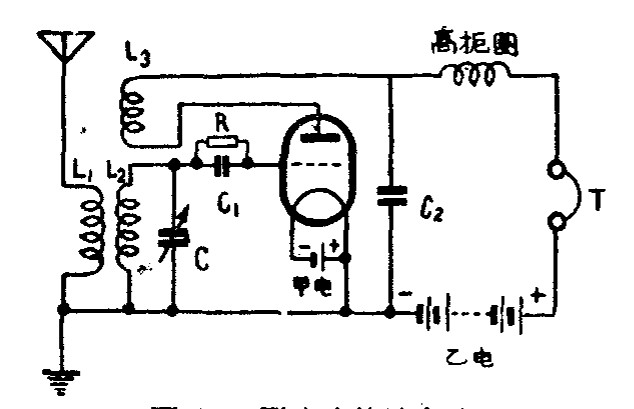
\includegraphics[width=0.9\linewidth]{regenerative_circuit.jpg}
    \caption{再生式检波电路}
    \label{fig:regenerative_circuit}
\end{figure}

在图\ref{fig:regenerative_circuit}中，屏极电路的高频扼流线圈（高扼圈）用于防止高频电流流入耳机。高频电流可以通过旁路电容器$C_2$形成回路，从而使再生过程更加稳定。

\section{再生的作用}

再生的主要作用包括：

\begin{enumerate}
    \item \textbf{提高灵敏度}：通过正反馈增强微弱信号，使收音机能够接收更远距离的电台
    \item \textbf{提高选择性}：增强谐振回路的Q值，使调谐更加尖锐
    \item \textbf{增加放大倍数}：反馈信号与输入信号叠加，等效提高了放大能力
\end{enumerate}

\section{再生的控制}

要使再生加大，可以采用以下方法：
\begin{enumerate}
    \item 增加再生线圈$L_3$的圈数；
    \item 缩短$L_2$和$L_3$的距离；
    \item 适当增加屏极电压（不超过规定值）。
\end{enumerate}

再生过强会导致收音机产生振荡电流的啸叫声，不仅无法正常收听，还会从天线上发射出电磁波，干扰附近收音机在相近频带的接收。因此，再生必须加以控制。

收音时，将再生调到将要发生振荡的临界点，此时灵敏度和选择性最佳，声音也最清晰宏亮，这一点称为再生的"临界点"。

再生程度需要适当控制：

\begin{description}
    \item[弱再生] 再生不足，灵敏度提升有限
    \item[临界再生] 接近振荡点，灵敏度和选择性最佳
    \item[强再生] 进入振荡状态，产生自激干扰
\end{description}

通常使用零件节省而效率较高的控制再生的方法有以下几种，各有优缺点：

\subsection{机械调节法}

通过机械变动再生线圈和调谐线圈的距离来控制再生。此法比较简单，但不够稳定，现在很少采用。

\subsection{可变电容器法}

使用可变电容器来控制再生，是最被广泛采用的方法。这是因为它的调谐细致，且可变电容器的机械性能很耐用。

\section{串连式再生与并联式再生}

根据再生线圈连接方式的不同，再生电路主要分为两种类型：

\subsection{串连式再生}

图\ref{fig:series_shunt_regeneration}甲的电路称为"串连式再生"。再生线圈$L_3$串联在屏极电路内，控制再生的可变电容器$C_2$并联在再生线圈的末端和电路零点间。残余高频经过$L_3$后，受到高频扼流圈的阻碍，从$C_2$通过；这样，增减$C_2$的电容量，就能控制通过$L_3$的高频电流，从而使再生受到控制。$C_2$通常称为"再生电容器"。

串连式再生电路的特点是：高频扼流圈有时可以省去不用（因为耳机里的线圈对高频电流也有扼流作用），但是$C_2$的容量要用得大一点，通常是0.00035微法。

\subsection{并联式再生}

图\ref{fig:series_shunt_regeneration}乙是"并联式再生"，再生线圈$L_3$和屏极电路并联；残余高频电流经过$L_3$和$C_2$自成一个回路，受到$C_2$的控制；音频电流则经由高扼圈和耳机等完成回路。因为高扼圈的接入，可以使高频和音频两种电流顺利分路。

并联式再生电路的特点是：$C_2$的电容量可以用得小一点，通常是0.0001微法；高扼圈如果省去，再生力就不够稳定。

\begin{figure}[htbp]
    \centering
    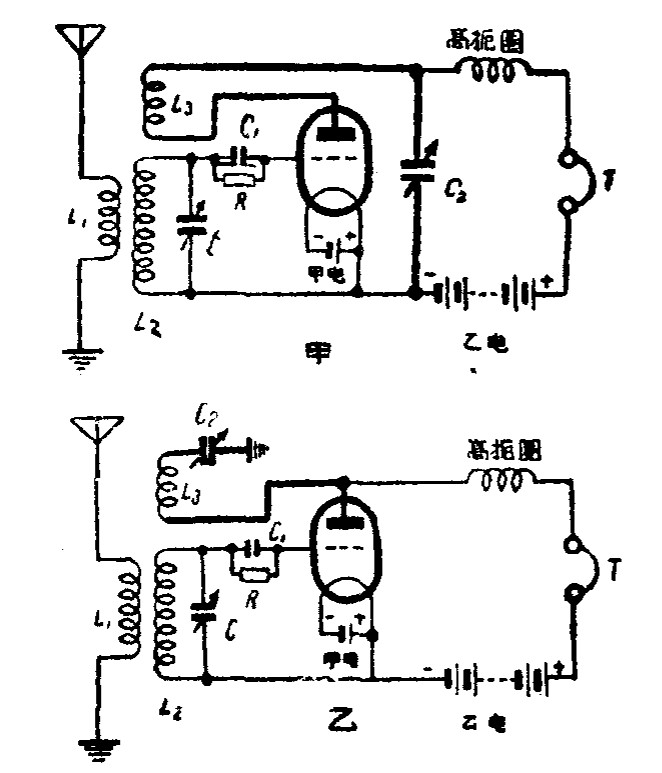
\includegraphics[width=0.9\linewidth]{series_shunt_regeneration.jpg}
    \caption{串连式再生（甲）与并联式再生（乙）电路}
    \label{fig:series_shunt_regeneration}
\end{figure}

\subsection{变动电源电压控制再生}

变动电源电压也可以控制再生。图\ref{fig:voltage_regeneration}就是这样的电路：屏极从并联在乙电上的电位器$R_1$取得可以变动的电压；电压高低就可以增减再生程度。这种方法实际上是通过控制电子管内部的电子流来影响再生的，所以效率也很好。$R_1$的阻值约为50千欧——100千欧，因为在它上面经常有电流通过，所以需要优良质量的电位器，否则很容易烧毁。

\begin{figure}[htbp]
    \centering
    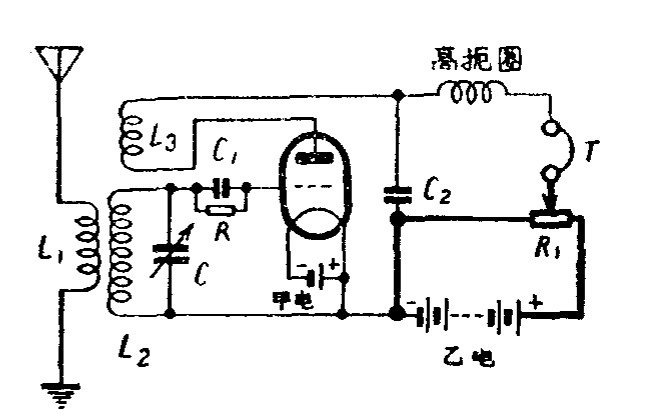
\includegraphics[width=0.7\linewidth]{voltage_regeneration.jpg}
    \caption{变动电源电压控制再生电路}
    \label{fig:voltage_regeneration}
\end{figure}

\subsection{帘栅电压控制再生}

用帘栅电子管作检波工作时，变动帘栅电压来控制管内的电子流，就能更有效地控制再生力。图\ref{fig:screen_grid_regeneration}就是这种电路的装置。将一只电位器$R_1$接入帘栅通向电源的电路上，固定电阻$R_2$是为了防止$R_1$旋到尽头时，避免帘栅受到过高的电压而设，有时可以省掉。当变动$R_1$的阻值时，帘栅上就有不同的电压，使电子流随着增减，再生便受到控制了。$C_3$是帘栅的旁路电容器，使帘栅上的交流成份从它那里流回阴极，不致在帘栅电路里引起交流电压降，影响收音质量，同时对帘栅电压起着稳定作用。

\begin{figure}[htbp]
    \centering
    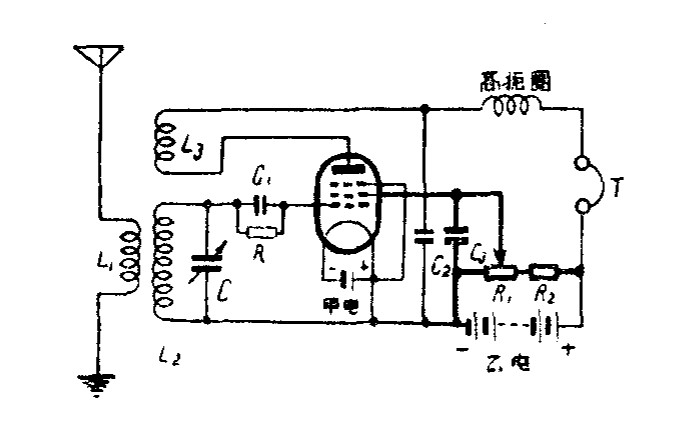
\includegraphics[width=0.9\linewidth]{screen_grid_regeneration.jpg}
    \caption{帘栅电压控制再生电路}
    \label{fig:screen_grid_regeneration}
\end{figure}

一般使用时，$R_1$的阻值常用50千欧，$R_2$为20-50千欧，$C_3$是0.05微法。

这样控制再生的方法非常平稳，效率可算优良，很受人们喜欢。

上面两种电路（变动电源电压控制和帘栅电压控制），再生圈也可以接成并联再生式。

\subsection{电位器并联控制再生}

将电位器并联在再生线圈的两端，使高频电流有一部分从它上面通过。变动电位器时，再生线圈里的电流也将受到影响；这样控制再生的方法也比较平稳。$R_1$的阻值通常是10千欧（图\ref{fig:potentiometer_shunt_regeneration}）。

\begin{figure}[htbp]
    \centering
    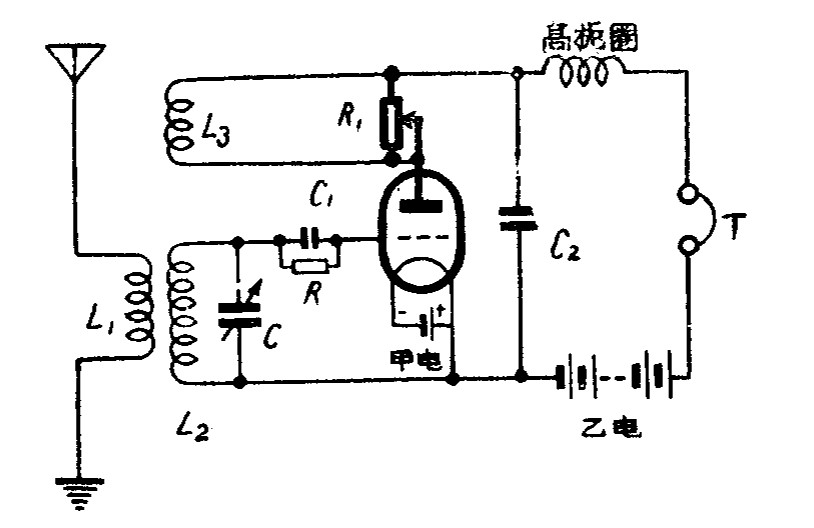
\includegraphics[width=0.7\linewidth]{potentiometer_shunt_regeneration.jpg}
    \caption{电位器并联控制再生电路}
    \label{fig:potentiometer_shunt_regeneration}
\end{figure}

\chapter{术语表}

\begin{description}
    \item[矿石检波器] 早期无线电接收装置中使用的检测器件
    \item[热电子发射] 金属被加热到炽热状态时表面释放电子的现象，也称爱迪生效应
    \item[真空二极管] 基于热电子发射原理制成的具有单向导电性的电子器件
    \item[直热式阴极] 灯丝本身直接发射电子的阴极结构
    \item[旁热式阴极] 灯丝加热、氧化物阴极发射电子的分离式阴极结构
    \item[单向导电性] 电流只能单向流动的特性
    \item[弗莱明阀] 弗莱明发明的真空二极管
    \item[控制栅极] 位于三极管阴极和阳极之间的金属丝网电极
    \item[真空三极管] 具有放大功能的真空电子器件
\end{description}

\backmatter

\begin{thebibliography}{99}
\addcontentsline{toc}{chapter}{参考文献}
\item 冯报本 编著. 单管收音机[M]. 北京: 人民邮电出版社, 1957.
\end{thebibliography}

\end{document}